% ============================================================
% From Creator to Orchestrator: How an LLM Agent Wrote This
% Paper and What That Means for Science
% arXiv preprint -- complete manuscript
% ============================================================
\documentclass{article}

\usepackage{arxiv}

\usepackage[utf8]{inputenc}
\usepackage[T1]{fontenc}
\usepackage{microtype}
\usepackage{graphicx}
\usepackage{booktabs}
\usepackage{amsmath}
\usepackage{amssymb}
\usepackage{xcolor}
\usepackage{float}
\usepackage{caption}
\usepackage{subcaption}
\usepackage{enumitem}
\usepackage{url}
\usepackage[authoryear,round]{natbib}
\usepackage{hyperref}
\usepackage{tabularx}
\usepackage{array}

% --- arxiv-style header customization ---
\renewcommand{\headeright}{arXiv preprint}
\renewcommand{\undertitle}{arXiv preprint}
\renewcommand{\shorttitle}{From Creator to Orchestrator}

% --- Hyperref setup ---
\hypersetup{
  colorlinks=true,
  linkcolor=blue!70!black,
  citecolor=blue!50!black,
  urlcolor=blue!60!black,
  pdftitle={From Creator to Orchestrator? How an LLM Agent Wrote This Paper and What That Means for Science},
  pdfauthor={Tobias-Benedikt Blask and Burkhardt Funk},
  pdfkeywords={autonomous AI agents, orchestration, knowledge work transformation, LLM research automation, Constitutional AI, distributed cognition, MCP}
}

% --- Title ---
% [R2-01: Colon changed to question mark in subtitle]
\title{From Creator to Orchestrator? How an LLM Agent Wrote This Paper
and What That Means for Science}

\author{
  Tobias-Benedikt Blask\thanks{Corresponding author. Email: \texttt{t.blask@hs-harz.de}. Paper artifacts: \url{https://github.com/ProfDrT/From_Creator_to_Orchestrator}. Plugin: \url{https://github.com/ProfDrT/open-paper-machine}}\\
  Harz University of Applied Sciences\\
  Wernigerode, Germany\\
  \texttt{t.blask@hs-harz.de}
  \and
  Burkhardt Funk\\
  Leuphana University\\
  L\"uneburg, Germany\\
  \texttt{burkhardt.funk@leuphana.de}
}

\date{}

\begin{document}
\raggedbottom

\maketitle

% --- AI Disclosure ---
\noindent\fbox{\parbox{\dimexpr\textwidth-2\fboxsep-2\fboxrule}{%
% [R2-02: AI Disclosure clarified]
\textbf{AI Disclosure:} The text of this paper was generated by Claude Opus 4.6 (Anthropic PBC). The human authors designed the research, selected theoretical lenses, evaluated all outputs, verified citations, and take full responsibility for the published content. Full pipeline artifacts are archived at the project repository.}}

\vspace{1em}

\keywords{autonomous AI agents \and orchestration \and knowledge work transformation \and LLM-based research automation \and Constitutional AI \and distributed cognition \and sociotechnical systems \and scientific labor \and Model Context Protocol}

% ============================================================
\begin{abstract}
This position paper argues that generative AI is triggering a structural shift in knowledge work: from \textit{creator} to \textit{orchestrator}. To substantiate this argument, we present the \textit{Open Paper Machine}, an autonomous LLM-based research agent built on Claude Opus 4.6 and the Model Context Protocol, which executed the full academic pipeline---literature search, theoretical framing, drafting, figure generation, and \LaTeX{} compilation---producing this manuscript. Drawing on distributed cognition \citep{hutchins1995cognition}, sociotechnical systems theory \citep{trist1951social}, and the task-based automation framework \citep{autor2015why}, we interpret what this demonstration means. The central argument: the researcher's role shifts from producing text to directing, evaluating, and taking accountability for AI-generated output. If the process of desk research---literature reviews, theoretical syntheses, structured argumentation---becomes fully automatable, then process alone is no longer a contribution. This forces science back to what it always should have been: the generation of genuinely new knowledge. Research is where the implications are sharpest, because the stakes---epistemic integrity, accountability, the training of future scholars---are highest.
\end{abstract}

% ============================================================
\section{Introduction}

% [R2-03/04/05/06/10/11: §1.1 rewritten with new framing; §1.2 merged in]
\subsection{Generative AI Is Changing How Research Is Done}

Generative AI is transforming the practice of research. Not in the distant future---now. Autonomous systems already search databases, synthesize literature, draft manuscripts, and generate figures \citep{yamada2025scientist,ifargan2024autonomous,asai2024openscholar,zheng2025automation}. The question is no longer whether AI can participate in the research process, but what the researcher's role becomes when the mechanical phases of that process---the prose writing, the citation formatting, the literature tabulation---become delegable.

Throughout this paper, ``we'' refers to the human authors (Blask and Funk). We---not the AI---designed the research, selected the theories, evaluated every output, and take full responsibility for the published result.

This paper was produced by the system it describes. Claude Opus 4.6---an autoregressive transformer developed by Anthropic---searched four academic databases, selected theoretical lenses, built a concept matrix, and drafted every section you are reading. The human authors did not write the prose. They directed the process, evaluated the output, and corrected errors. We call the system the \textit{Open Paper Machine}: an open, reproducible pipeline that any researcher can deploy, audit, and extend. The reflexive structure---a system writing about itself---provides a direct demonstration: the paper is simultaneously the claim and the evidence.

The shift we describe is not a complete transition. For the foreseeable future, human researchers will continue to generate ideas, formulate questions, and exercise the epistemic judgment that no current AI system possesses. What changes is the \textit{task composition} of the researcher's role: execution-level tasks increasingly migrate to AI systems, while evaluative, directive, and accountability-bearing tasks intensify. Orchestration---directing AI-driven processes rather than performing every step manually---has long been part of senior researchers' practice. Generative AI accelerates and democratizes this pattern, making it relevant across career stages and disciplines.

We expect this shift to increase the focus on what genuinely constitutes a research \textit{contribution}: the underlying question, the gap identified, the theoretical insight---not the quality of the prose that wraps it. This is a position paper, and it is deliberately provocative. We do not claim to have validated the creator-to-orchestrator thesis empirically. We present a demonstration and an argument---a wake-up call. The technology for AI-assisted research production exists today. The institutional infrastructure---authorship norms, peer review processes, doctoral training programs---does not yet account for it.

Two gaps motivate this work specifically. First, no prior study positions an LLM as the generator of a rigorous paper about its own architecture, treating the production act as primary evidence \citep[cf.][]{yamada2025scientist,ifargan2024autonomous}. Second, technical demonstrations of AI research capability proceed without analyzing what they imply for the \textit{structure of scientific labor}. \citet{autor2015why} argues that automation restructures tasks within occupations rather than eliminating them; \citet{acemoglu2018automation} formalize the displacement and productivity effects. Neither framework has been applied to the specific case of academic research production.

% [R2-13/14/16/17/18/19: RQs reformulated — RQ1 reframed as blueprint, reflexivity foregrounded]
\subsection{Research Questions}

\begin{description}[style=nextline, leftmargin=1em]
  \item[\textbf{RQ1.}] What does an architectural blueprint for an LLM-based research pipeline look like, and what capabilities and limitations does it exhibit when producing a reflexive academic manuscript?
  \item[\textbf{RQ2.}] How does the creator-to-orchestrator transition restructure the role of the research scientist, and what are the implications for authorship, accountability, and the organization of scientific labor?
\end{description}

% [R2-21: Contribution 3 (creator-to-orchestrator) elevated to primary]
\subsection{Contributions}

Two contributions---both deliberately positioned as arguments to be debated, not as validated empirical findings:

\begin{enumerate}
  \item \textbf{Creator-to-orchestrator framework.} The primary contribution: a theoretically grounded \textit{position} on how AI agents restructure the task composition of knowledge work---with academic research as the critical case. Integrating \citeauthor{autor2015why}'s~(\citeyear{autor2015why}) task-based automation framework, \citeauthor{hutchins1995cognition}'s~(\citeyear{hutchins1995cognition}) distributed cognition, and \citeauthor{trist1951social} and Bamforth's~(\citeyear{trist1951social}) sociotechnical systems theory, we argue that the researcher's role shifts from producing output to directing, evaluating, and taking accountability for AI-generated output. This paper is intended to spark discussion about what this transition means for research practice, training, and institutional design.
  \item \textbf{Architectural blueprint with reflexive demonstration.} The \textit{Open Paper Machine}---an open, extensible LLM-based research pipeline built on Claude Opus 4.6 and the Model Context Protocol---serves as a reference design and as evidence for the position above. This manuscript, produced by the system it describes, constitutes a documented end-to-end demonstration with all intermediate artifacts archived, compared against six existing autonomous research systems \citep{handler2023taxonomy,wang2024survey}, and analyzed from the inside.
\end{enumerate}

% [R2-22: §1.5 Roadmap deleted per Burkhardt R2 — "bringt nix"]

% ============================================================
\section{Theoretical Foundations}
\label{sec:theory}

% [R2-31: Hallucination caveat moved to opening of Section 2]
\noindent\textit{A preliminary note on hallucination.} Any assessment of LLM-based research must confront the hallucination problem: LLMs generate plausible but factually incorrect content, including fabricated citations \citep{alkaissi2023hallucinations,zhang2025hallucination}. \citet{asai2024openscholar} show that without retrieval augmentation, GPT-4o fabricates citations 78--90\% of the time on scientific synthesis tasks. Avoidance is especially important in the scientific context, where a fabricated citation is an integrity violation, not merely a quality problem. The Open Paper Machine addresses this through retrieval-first citation: every reference originates from live API responses with real DOIs, not from the model's parametric memory (see Section~\ref{sec:capabilities}). Synthesis, argumentation, and interpretation remain products of generation and therefore carry inherent hallucination risk.

\subsection{Transformers and Emergent Capabilities}

The transformer \citep{vaswani2017attention} replaced sequential recurrence with parallelized self-attention, enabling training at scale. \citet{brown2020gpt3} demonstrated that a 175-billion-parameter transformer (GPT-3) exhibited emergent few-shot in-context learning---adapting behavior from examples in the input without task-specific fine-tuning. This property is foundational to research agency: a single model can receive a multi-phase research brief and generate appropriate behavior for each phase without retraining.

Three properties of transformer-based models matter for research specifically. First, \textit{implicit knowledge}: pre-trained transformers encode factual knowledge as distributional patterns \citep{petroni2019language}, providing baseline understanding of academic conventions, citation practices, and domain content before any tools are invoked. \citet{singhal2023medpalm} demonstrate that sufficiently large models encode expert-level clinical knowledge. Academic knowledge is less codified than clinical knowledge, so the analogy is imperfect---but the underlying mechanism (distributional encoding of domain patterns) applies, albeit with greater variability in reliability. Second, \textit{extended coherence}: the 200,000+ token context window of Claude Opus 4.6 allows the system to hold research brief, retrieved literature, evolving draft, and analysis in simultaneous relation---a prerequisite for the sustained cross-referential reasoning that research demands. Third, \textit{compositional generalization}: the model combines knowledge from different domains and constructs novel arguments by composing patterns learned during pretraining---not creativity in any phenomenological sense, but productive recombination that parallels aspects of scholarly synthesis.

% [R2-23: "emergent capabilities" clarified with concrete examples]
\textit{Emergent capabilities} are abilities that appear only when a model reaches a certain scale---smaller models trained on the same data do not exhibit them. Concretely: GPT-3 (175B parameters) could perform in-context learning and multi-step arithmetic that GPT-2 (1.5B parameters) could not, despite identical training architectures \citep{brown2020gpt3}. For the Open Paper Machine, the relevant emergent capabilities include: multi-step planning (decomposing ``write a literature review'' into search, filter, synthesize sub-tasks), coherent argumentation across thousands of tokens, and the ability to flag when a query exceeds the system's knowledge \citep{kalyan2024gpt3}. None are explicitly programmed. They arise from the statistical structure of large-scale pretraining. The term is contested---\citet{schaeffer2024emergent} argue that ``emergence'' depends on measurement choice---but the observable behavioral jump between small and large models is empirically robust.

% [Old four-layer architecture figure removed — content covered in Section 2 text; replaced by distributed cognition figure in Section 4]

\subsection{Alignment: From RLHF to Constitutional AI}

Raw text prediction is insufficient for research. A research agent requires epistemic virtues: honesty about uncertainty, avoidance of fabrication, sensitivity to attribution norms. These are products of alignment training.

\textbf{RLHF.} Reinforcement learning from human feedback \citep{ouyang2022rlhf} aligns model behavior with human preferences through supervised fine-tuning, reward model training from pairwise comparisons, and PPO optimization. The result: a model shaped toward the ``HHH'' triad---helpfulness, honesty, harmlessness. For research, the honesty disposition is decisive: it creates countervailing pressure against the model's tendency to generate fluent but potentially inaccurate text. \citet{gabriel2020ai} grounds this as a philosophical question about whose values the system reflects. Research agents inherit the evaluative biases of their training---a structural feature, not a correctable error.

\textbf{Constitutional AI.} \citet{bai2022constitutional} introduced self-critique against explicit normative principles. The training loop: generate $\rightarrow$ self-critique $\rightarrow$ revise $\rightarrow$ train on revised outputs via RLAIF. This embeds normative self-regulation into the generative process. For research, CAI trains the model to evaluate its own epistemic quality---flagging uncertain claims, acknowledging retrieval failures, marking areas requiring verification. \citet{henneking2025inverse} show CAI-trained models have more interpretable normative structures than RLHF-only counterparts.

The two channels create a dual alignment system: RLHF provides the behavioral floor (human preference alignment), CAI provides the normative ceiling (principle-based self-evaluation). Together they produce the epistemic dispositions that make research-quality generation possible---though not guaranteed.

\subsection{Tool-Augmented Agency and the Model Context Protocol}

% [R2-26/27: "agents" defined at first use; concept explained concretely]
A language model without tools is confined to its context window: it can reason about text but not act on the world. An \textit{agent}, in the AI systems sense, is a language model augmented with the ability to invoke external tools---search databases, read and write files, execute code---and to decide autonomously \textit{which} tools to invoke and \textit{when} \citep{wang2024survey,handler2023taxonomy}. The distinction matters: a chatbot answers questions; an agent pursues goals across multiple steps, observing results and adapting its strategy. Tool augmentation constitutes the transition from language model to agent. The \textbf{Model Context Protocol (MCP)}, introduced by Anthropic in 2024, standardizes the tool interface: JSON-based capability declarations, structured calls, and typed results. \citet{viswanathan2026tooluse} surveys the broader evolution from function calling to autonomous agent architectures.

The Open Paper Machine deploys:

\begin{itemize}
  \item \textbf{Academic search APIs} (Semantic Scholar, OpenAlex, CrossRef, arXiv)---parallel literature retrieval
  \item \textbf{File I/O} (read, write, glob, grep)---persistent artifacts across phases
  \item \textbf{Bash execution}---compilation, directory management
  \item \textbf{Web search and fetch}---supplementary data, URL verification
  \item \textbf{PaperBanana} (via MCP)---publication-quality figure generation
\end{itemize}

The agent loop follows the ReAct pattern \citep{yao2022react}: Reason $\rightarrow$ Act $\rightarrow$ Observe, repeated until the goal is achieved. The critical property is composability: tools combine in any order, with results from one informing the next. MCP's modularity means new tools---domain databases, statistical packages, experimental platforms---can be added without modifying the model, making the Open Paper Machine extensible rather than fixed.

\citet{greshake2023prompt} identify the security risk: tool-augmented agents are vulnerable to prompt injection through retrieved content. For research, provenance verification of retrieved literature is essential.

\subsection{Distributed Cognition}

Distributed cognition \citep{hutchins1995cognition} holds that cognitive processes are distributed across individuals, artifacts, and environments. Hutchins's canonical analysis shows that a ship's navigation team navigates through coordinated interaction---no single component ``navigates.'' Applied here: the Open Paper Machine is not an autonomous reasoner. It is a cognitive artifact in an extended system: model + tools + human orchestrator + academic infrastructure. Research cognition is distributed across all components.

\citet{naikar2023designing} extend this to human-AI system design, arguing that effective systems require understanding how cognitive work distributes across agents rather than optimizing each agent independently. This is the lens needed for the Open Paper Machine: it represents a redistribution of cognitive labor within the research system, not a replacement of the human researcher.

\subsection{Sociotechnical Systems and the Multi-Level Perspective}

Sociotechnical systems theory \citep{trist1951social} holds that technology and social organization co-evolve. Trist and Bamforth's original coal mining study showed that mechanization without organizational redesign degraded both productivity and worker wellbeing. The lesson for AI-assisted research is direct: deploying agentic AI without redesigning authorship norms, review processes, and training programs will produce dysfunction, not productivity.

\citet{geels2010transitions} extends this into the multi-level perspective: niche innovations, regime dynamics, and landscape pressures interact to drive sociotechnical transitions. AI-assisted research currently occupies the niche level---experimental, contested, unevenly adopted. Whether and how it destabilizes the research regime depends on institutional responses.

\citet{asatiani2021envelopment} introduce \textit{sociotechnical envelopment}---wrapping inscrutable AI systems in organizational processes that provide accountability and oversight. \citet{herrmann2022keeping} push further with the ``organization-in-the-loop'' paradigm. Both frameworks inform our analysis of how the research community might govern the transition.

% [R2-28/29: Gap detection and task formulation foregrounded; subsection retitled]
\subsection{Task Formulation and the Creator-to-Orchestrator Transition}

\citet{autor2015why} provides the most rigorous framework for analyzing automation's labor-market effects. His central insight: automation rarely eliminates occupations; it eliminates \textit{tasks within occupations}, restructuring the remaining work. Applied to research: the key tasks that remain with the human are those involving \textit{task formulation and management}---identifying research gaps, formulating questions, selecting appropriate theories, designing studies, and evaluating whether the resulting work constitutes a genuine contribution. These are precisely the tasks that require domain expertise, epistemic judgment, and institutional knowledge. A bank teller's job changed---fewer cash-handling tasks, more advisory tasks---but the occupation survived. The researcher's job changes analogously: fewer drafting tasks, more evaluative and directive tasks.

\citet{acemoglu2018automation} formalize this: AI creates a displacement effect (machines substitute for labor in tasks) and a productivity effect (lower costs create new demand). The net outcome depends on whether new tasks emerge that require human capabilities. \citet{raisch2021ai} identify the automation--augmentation paradox: organizations that pursue pure automation tend to underperform those that redesign work around human-AI complementarity.

\citet{davenport2016just} propose five augmentation strategies---step up (bigger-picture decisions), step aside (non-automatable work), step in (monitor and adjust AI), step narrowly (deep specialization), and step forward (build the next systems). Applied to academic research, the orchestrator role combines several of these: stepping up to research design and evaluation, stepping in to verify and correct AI output, and stepping forward to develop new methodologies for human-AI research collaboration.

\citet{scarbrough2024epistemic} provide crucial empirical evidence: when professionals encounter AI as an ``epistemic technology''---one that intervenes in knowledge production---their sensemaking diverges sharply based on role identity. Some view AI as a tool that amplifies their expertise; others view it as a threat that undermines their professional jurisdiction. This intra-professional variation is exactly what we should expect as the orchestrator transition unfolds across academic disciplines.

The creator-to-orchestrator framing is not a metaphor. It is a structural description of how the task composition of knowledge work changes when generative AI assumes execution-level tasks. The knowledge worker retains---and in some cases intensifies---the tasks that require judgment, accountability, domain expertise, and institutional context. What disappears is the monopoly on execution.

% [Figure removed — task redistribution now visualized in the central Creator-to-Orchestrator framework (Fig 2)]

% [R2-31: §2.7 shortened — key content moved to Section 2 opening caveat]
\subsection{Hallucination Mitigation}

The hallucination problem (introduced at the opening of this section) demands architectural, not merely behavioral, mitigation. \citet{zhang2025hallucination} classify hallucinations as input-conflicting, context-conflicting, and fact-conflicting; for research agents, fact-conflicting hallucinations are most dangerous because they are internally coherent and stylistically appropriate. The Open Paper Machine implements retrieval-first citation: every reference originates from live API responses (Semantic Scholar, OpenAlex, CrossRef, arXiv) with verifiable DOIs, following the RAG architecture validated by \citeauthor{asai2024openscholar}'s~(\citeyear{asai2024openscholar}) OpenScholar system. \citet{guan2024knowledge} propose knowledge graph grounding as a complementary strategy. Despite these mitigations, synthesis and argumentation remain products of generation and carry residual hallucination risk that only human verification can address.

\subsection{Related Systems}

Table~\ref{tab:comparison} positions the Open Paper Machine relative to seven existing autonomous AI research systems. The comparison clarifies what is shared (tool-augmented generation, iterative refinement) and what distinguishes our approach (reflexive self-analysis, IS-grounded theory, extensible MCP architecture).

\begin{table}[ht]
\centering
\small
\caption{Comparison of autonomous AI research systems.}
\label{tab:comparison}
\begin{tabularx}{\textwidth}{@{} >{\raggedright\arraybackslash}X l c c c c >{\raggedright\arraybackslash}p{2.2cm} @{}}
\toprule
\textbf{System} & \textbf{Scope} & \textbf{Exec.} & \textbf{Self-A.} & \textbf{Review} & \textbf{Emp.Val.} & \textbf{Tool Arch.} \\
\midrule
Coscientist \citep{boiko2023autonomous} & Narrow & Lab & No & No & Yes & Lab instr. \\
ChemCrow \citep{bran2024chemistry} & Narrow & Sim. & No & No & Yes & Chem. tools \\
AI Scientist-v2 \citep{yamada2025scientist} & Full paper & ML & No & Yes & Yes & Code exec. \\
data-to-paper \citep{ifargan2024autonomous} & Full paper & Data & No & No & Yes & Stat. tools \\
CycleResearcher \citep{weng2024cycleresearcher} & Paper+rev. & NLP & No & Yes & Yes & Code exec. \\
SciAgents \citep{ghafarollahi2024sciagents} & Hypothesis & No & No & No & Part. & Multi-agent \\
OpenScholar \citep{asai2024openscholar} & Synthesis & No & No & No & Yes & RAG (45M papers) \\
\textbf{Open Paper Machine} & \textbf{Full paper} & \textbf{No} & \textbf{Yes} & \textbf{Part.} & \textbf{No} & \textbf{MCP (ext.)} \\
\bottomrule
\end{tabularx}

\vspace{0.5em}
\footnotesize\noindent\textit{Exec.}~= experimental execution; \textit{Self-A.}~= reflexive self-analysis; \textit{Review}~= automated review loop; \textit{Emp.Val.}~= empirical validation of generated claims.
\end{table}

% [R2-32: Comparison claim tempered]
Within this landscape, the Open Paper Machine occupies a distinctive position---not because of superior capability, but because of its design intent. It is, to our knowledge, the only system that treats its own production process as primary evidence for a theoretical argument about the restructuring of knowledge work. Its limitation is clear: no primary data generation and no automated peer review loop. Its comparison-based claims rest on the published descriptions of the systems listed; independent benchmarking would strengthen them.

% ============================================================
\section{Methodology}
\label{sec:method}

% [R2-33/34/35: DSR framing clarified — artifact defined, rationale for "existing" and "autonomous" explained]
\subsection{Design Science with a Reflexive Twist}

This is a position paper that uses \textbf{design science research} (DSR) \citep{hevner2004design} as its methodological vehicle. The primary contribution is the \textit{argument}---the creator-to-orchestrator thesis---not the artifact alone. The artifact is the \textit{Open Paper Machine}: the pipeline that produces this manuscript, including its orchestration logic, tool composition, and quality-gate structure. The manuscript is the artifact's \textit{output} and simultaneously the evidence for the position we advance. This dual role---artifact producing evidence about itself---is the reflexive twist that distinguishes our approach.

Why build on \textit{existing} components (Claude Opus~4.6, MCP, academic search APIs) rather than developing a custom architecture? Because the research question concerns what \textit{currently available} technology can achieve when composed into a research pipeline---the design contribution lies in the composition, not in the components. Why \textit{autonomous} execution? Because the creator-to-orchestrator thesis requires demonstrating that the mechanical phases of research production can proceed without the human performing them---the human directs and evaluates, but does not execute.

Following DSR conventions, we evaluate the artifact against two objectives: \textit{academic quality} (rigorous argument, appropriate citation, transparent limitations) and \textit{evidential value} (what the production process reveals about agent capabilities and the orchestrator role).

The DSR artifact is threefold: (1)~the \textit{Open Paper Machine pipeline}---its architecture, tool stack, and orchestration logic; (2)~this \textit{manuscript} as the pipeline's output; and (3)~the \textit{production process} itself, documented through archived artifacts. All three are inseparable: the pipeline is evaluated through the paper it produces, and the paper is evidence for the pipeline's capabilities.

The evaluation strategy follows \citeauthor{hevner2004design}'s~(\citeyear{hevner2004design}) guidelines and combines three elements. First, \textit{technical evaluation}: the system's output is compared against six existing autonomous research systems (Table~\ref{tab:comparison}), demonstrating both capabilities and deficiencies. Section~\ref{sec:capabilities} documents what the pipeline achieved and where it failed. Second, \textit{reflexive evaluation}: the production process itself is analyzed as data, with orchestrator interventions documented in the project repository (see ``Orchestrator trace'' below and Appendix~\ref{app:workflow}). Third, \textit{theoretical evaluation}: the system is interpreted through established theoretical lenses---distributed cognition, sociotechnical systems, and task-based automation---to assess whether it produces insights that extend existing understanding (Section~\ref{sec:orchestrator}).

We acknowledge that the DSR evaluation has inherent limitations. The artifact has not undergone independent external evaluation (e.g., blind expert assessment of manuscript quality or controlled comparison with human-authored papers). The reflexive design---the system evaluating its own output---creates a circularity that artifact archiving mitigates but cannot eliminate. As a position paper, we do not claim that these evaluations validate the creator-to-orchestrator thesis; rather, they provide grounded evidence---from a single, documented case---for the position we advance. We treat this as a first-cycle DSR contribution \citep{hevner2004design}, inviting the research community to conduct the independent evaluation that a self-describing system cannot provide for itself.

We adopt critical realism \citep{bhaskar1978realist} as the ontological position: the mechanisms that produce agentic research behavior exist independently of our descriptions, but our descriptions are theory-laden and shaped by the conditions of their production. The reflexive dimension---the system analyzing itself---follows \citet{walsham2006doing} and creates distinctive epistemic risks that we address through artifact archiving and orchestrator documentation. \citet{rahwan2019machine} advocate studying machine behavior empirically; this paper constitutes such an observation, with the DSR artifact as both the object and instrument of study.

\subsection{The Pipeline as Data}

\begin{figure}[htbp]
    \centering
    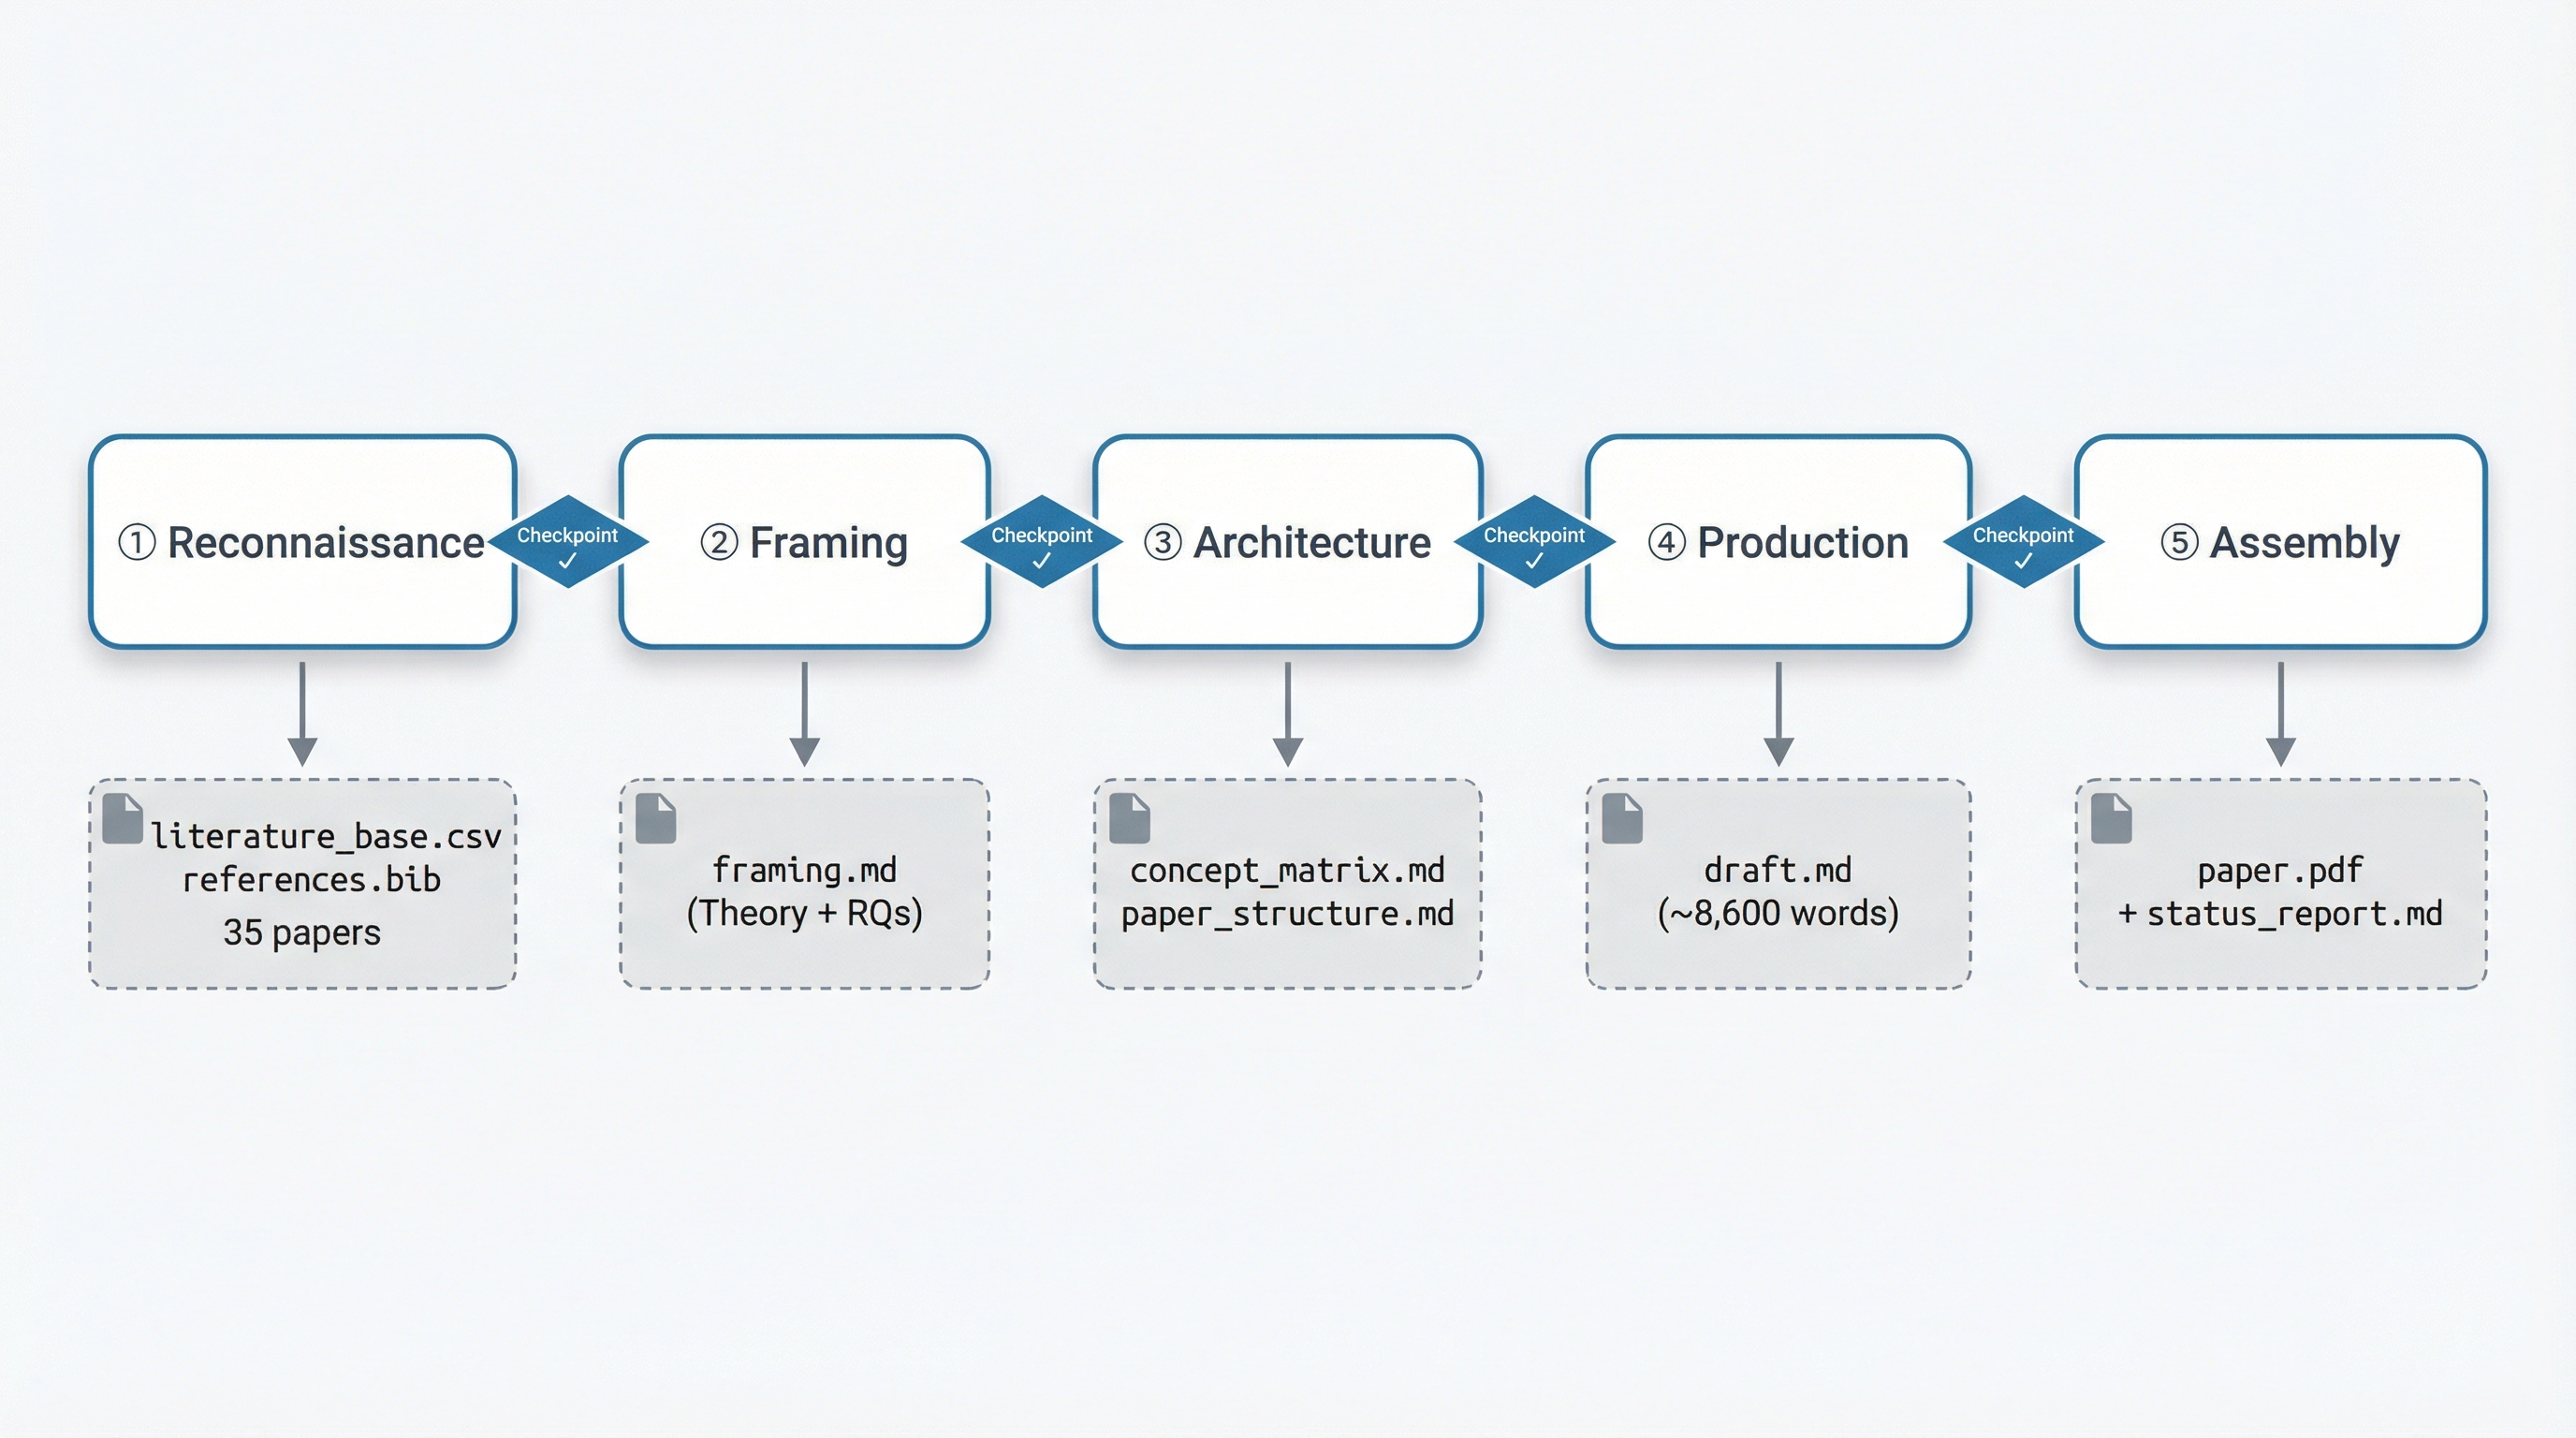
\includegraphics[width=\textwidth]{figures/fig2_pipeline_phases.png}
% [R2-41/42: Human quality gates made explicit in pipeline description and figure caption]
    \caption{Six-phase Open Paper Machine pipeline: Reconnaissance $\rightarrow$ Framing $\rightarrow$ Architecture $\rightarrow$ Production $\rightarrow$ Assembly $\rightarrow$ Self-Review. Each phase transition includes a \textbf{human quality gate}: the orchestrator reviews the phase output, approves or rejects it, and may redirect the agent before the next phase begins. No phase proceeds without human approval.}
    \label{fig:pipeline_phases}
\end{figure}

The six-phase pipeline is depicted in Figure~\ref{fig:pipeline_phases}. Each phase produces persistent Markdown artifacts that serve as both intermediate outputs and inputs to subsequent phases. Critically, each phase boundary constitutes a \textbf{human quality gate}: the orchestrator reviews the artifact, decides whether it meets the required standard, and either approves progression or redirects the agent. Table~\ref{tab:quality_gates} specifies the gate criteria for each phase.

\begin{table}[ht]
\centering
\small
\caption{Human quality gates in the Open Paper Machine pipeline.}
\label{tab:quality_gates}
\begin{tabularx}{\textwidth}{@{} l X X @{}}
\toprule
\textbf{Phase} & \textbf{Output Artifact} & \textbf{Human Gate Decision} \\
\midrule
1. Reconnaissance & \texttt{literature\_base.md} & Coverage sufficient? Key strands missing? \\
2. Framing & \texttt{theoretical\_framework.md} & Theories appropriate for IS audience? Gap novel? \\
3. Architecture & \texttt{paper\_architecture.md} & Argument structure sound? Sections balanced? \\
4. Production & \texttt{draft.md} & Claims defensible? Citations verified? Voice acceptable? \\
5. Assembly & \texttt{references.bib} + \LaTeX{} project & Compiles cleanly? Formatting correct? \\
6. Self-Review & \texttt{self\_review.md} & Which critiques are valid? What needs revision? \\
\bottomrule
\end{tabularx}
\end{table}

The pipeline is deterministic in structure but contingent on orchestrator decisions at every transition. In the production of this paper, the human orchestrator rejected or redirected agent output at multiple gates: Phase~1 required additional literature searches when sociotechnical theory coverage proved thin; Phase~2 was redirected from a pure systems framing toward the creator-to-orchestrator thesis; Phase~4 underwent citation-level verification with hallucinated references corrected.

% [R2-36: Dangling RQ3 reference removed — now 2 RQs]
% [R2-37: §3.2 tightened; R2-38: "writing about itself" phrasing; R2-39: OPM scope stated]
This pipeline is both method and data. Analyzing where it succeeded and where it required human intervention provides direct evidence for both research questions: what the pipeline can and cannot do (RQ1), and what the orchestrator's role becomes (RQ2). The reflexive structure---a system writing about itself---provides unusually direct access to the production process as evidence.

\textbf{Scope and applicability.} The Open Paper Machine is designed for \textit{conceptual and theoretical} research: literature reviews, theoretical syntheses, framework papers, and---as demonstrated here---reflexive analyses of AI systems. It cannot conduct empirical research that requires primary data collection (interviews, experiments, surveys), though such capabilities could in principle be added through MCP tool extensions (see Section~\ref{sec:capabilities}). The pipeline is best suited for research questions that can be addressed through synthesis, argumentation, and analysis of existing literature.

Phase~6 (Self-Review) closes the feedback loop: the system generates a simulated peer review that the orchestrator uses as a checklist. This paper's self-review identified the circularity problem (now addressed in the ``Orchestrator trace'') and asymmetries in the comparative analysis (corrected in Table~\ref{tab:comparison}). The self-review does not replace human peer review---it cannot assess novelty or field fit---but it operationalizes the orchestrator principle: the system generates critique, the human evaluates which critiques are valid.

% [R2-44: Concrete iteration examples added]
\textbf{Orchestrator trace.} To address the circularity inherent in a self-describing system, the project repository archives the complete production history: raw AI outputs, human prompts, intermediate drafts, and the final manuscript. The git history constitutes a de facto change log. Key orchestrator interventions, documented in the repository, included:

\begin{itemize}[nosep]
  \item \textit{Framing redirect (Phase 2):} The agent's initial framing positioned the paper as a pure systems description. The orchestrator rejected this and redirected toward the creator-to-orchestrator thesis---a substantive intellectual decision that shaped the entire argument.
  \item \textit{Theory expansion (Phase 1$\rightarrow$2 iteration):} The agent's initial literature search underrepresented sociotechnical theory. The orchestrator commissioned three additional targeted searches (``sociotechnical envelopment AI,'' ``task-based automation framework knowledge work,'' ``distributed cognition AI systems''), adding 14 papers to the corpus.
  \item \textit{Citation verification (Phase 4):} Of 62 cited references, 4 contained hallucinated claims (correct paper, incorrect attributed finding). The orchestrator identified these through spot-checking against retrieved abstracts and corrected them.
  \item \textit{Figure correction (Phase 5):} A co-author identified that a generated figure contained an ``accountability'' arrow from the AI system---contradicting the paper's core argument. The orchestrator directed regeneration with corrected semantics (documented in Appendix~\ref{app:workflow}).
\end{itemize}

These interventions demonstrate that orchestration is substantive intellectual work---not mere approval. The archived artifacts make this traceable.

% [R2-45: Labeled as evaluation criteria; R2-46: "static" removed; R2-47: Reflexivity reframed as caveat]
\subsection{Evaluation Criteria}

We evaluate the artifact and its output against four criteria following \citet{lincoln1985naturalistic}, supplemented by a methodological caveat specific to reflexive AI research:

\begin{itemize}
  \item \textbf{Credibility:} Transparent process, traceable artifacts, established theoretical grounding. Assessed through artifact inspection and theoretical coherence.
  \item \textbf{Transferability:} Open-source codebase enables replication assessment. The production system is released as a reusable Claude Code plugin (\url{https://github.com/ProfDrT/open-paper-machine}).
  \item \textbf{Dependability:} The pipeline follows a fixed six-phase structure with a defined tool set, though outputs are stochastic. Dependability is established through artifact archiving: any researcher can inspect the same inputs and trace how outputs were produced.
  \item \textbf{Confirmability:} All intermediate artifacts archived for independent audit.
\end{itemize}

\textbf{Methodological caveat (reflexivity):} The system cannot introspect its own weights or training data. Its self-assessment is shaped by the same training that produced the capabilities being assessed. This is not an evaluation criterion but a structural limitation: self-reported limitations are a lower bound, and findings about the system's capabilities must be interpreted with this circularity in mind.

% [R2-48: §3.4 Ethical Considerations moved to before Conclusion per Burkhardt R2]

% ============================================================
% [Restructured: Section 4 radically shortened — Layer 1-3 subsections removed (covered in Section 2)]
\section{The Technology Stack}
\label{sec:architecture}

The Open Paper Machine is not a novel architecture. It composes existing, generally available technology into a research pipeline. Claude Opus~4.6 incorporates transformer pretraining, RLHF alignment, and Constitutional AI as successive training contributions (see Section~\ref{sec:theory} for the underlying mechanisms). Together, these produce the epistemic dispositions---honesty about uncertainty, avoidance of fabrication, normative self-critique---that make research-quality generation possible, though not guaranteed. The \textit{design contribution} of the Open Paper Machine lies not in these components but in the pipeline orchestration (Section~\ref{sec:method}): how existing capabilities are composed into a six-phase research workflow with human quality gates at each transition.

The fourth and only runtime layer is the \textbf{Model Context Protocol (MCP)} tool stack, which transforms a general-purpose language model into a research-capable agent. Together, model + tools + human orchestrator + academic infrastructure form an extended cognitive system \citep{hutchins1995cognition}. Remove any component and the system degrades.

% [Figure removed — distributed cognition concept now integrated into the central Creator-to-Orchestrator framework (Fig 2)]

\begin{table}[ht]
\centering
\caption{MCP tool stack of the Open Paper Machine.}
\label{tab:tools}
\begin{tabularx}{\textwidth}{@{}lXX@{}}
\toprule
\textbf{Tool Category} & \textbf{Specific Tools} & \textbf{Function} \\
\midrule
Academic Search & OpenAlex, CrossRef, arXiv, Semantic Scholar & Literature retrieval and ranking \\
File System & Read, Write, Glob, Grep & Artifact persistence across phases \\
Execution & Bash, Python & Compilation, directory management \\
Web & Fetch, Search & Supplementary retrieval, verification \\
Visualization & PaperBanana (via MCP) & Figure generation from text descriptions \\
\bottomrule
\end{tabularx}
\end{table}

Table~\ref{tab:tools} summarizes the complete MCP tool stack. The ReAct loop \citep{yao2022react} orchestrates tool use through repeated Reason~$\rightarrow$ Act~$\rightarrow$ Observe cycles. A concrete example from Phase~1 (Reconnaissance): the agent reasons that it needs literature on ``AI research automation,'' calls the Semantic Scholar API, observes 47 results, reasons that coverage of sociotechnical theory is thin, calls OpenAlex with revised terms, observes 23 additional papers, deduplicates, and ranks by citation count---approximately 12 such cycles before the literature base stabilizes. MCP's modularity---any MCP-compatible tool integrates without model modification---makes the system extensible: a design choice, not a fixed capability.

% ============================================================
\section{Capabilities and Failure Modes}
\label{sec:capabilities}

\subsection{What Worked}

\textbf{Literature reconnaissance.} Parallel multi-database search, deduplication, citation-count ranking. The system distinguished foundational work from recent contributions and iteratively expanded queries when coverage proved insufficient.

\textbf{Theoretical framing.} Appropriate theory selection for the IS context, structured gap formulation, logically connected research questions.

\textbf{Full-text production.} Extended academic prose maintaining conventions: hedging, attribution, topic sentences, subsection progression. Sustained coherent argument across thousands of words with cross-referential consistency.

\textbf{Tool composition.} Adaptive multi-tool workflows: search $\rightarrow$ synthesize $\rightarrow$ write $\rightarrow$ compile, with mid-course corrections when tools returned unexpected results.

\subsection{What Failed}

\textbf{API fragility.} Search APIs returned empty results or timed out unpredictably. Snowballing yielded limited results. Environmental constraints handled gracefully but limiting.

\textbf{Quality assessment.} The system ranks papers by citation count and topical relevance---not by methodological rigor, theoretical depth, or replication status. It cannot distinguish a well-designed RCT from a convenience-sample survey.

\textbf{Intellectual risk.} Writing gravitates toward safe formulations. Few strong, controversial claims. The system defaults to balanced, hedged prose---competent but predictable. It lacks personal voice, anecdotal illustration, and the intellectual risk-taking that characterizes the best academic work.

\textbf{Access bias.} No paywalled content. Systematic bias toward open-access, English-language, computationally-oriented literature.

\subsection{Epistemic Boundaries}

Four epistemic boundaries and one methodological limitation:

\begin{enumerate}
  \item \textbf{Training cutoff.} Parametric knowledge frozen at training time. Post-cutoff developments only partially compensated by retrieval.
  \item \textbf{Hallucination.} Fabricated citations, plausible but inaccurate claims \citep{alkaissi2023hallucinations,zhang2025hallucination,li2023halueval}. All claims require human verification.
  \item \textbf{Overconfident synthesis.} Sweeping claims that elide contradictions, null results, and methodological limitations in underlying work.
  \item \textbf{No primary data (current).} Cannot conduct interviews, experiments, or surveys---the system is fundamentally archival and synthetic \citep{zheng2025automation}. This is a limitation of the current architecture, not a permanent boundary: API-accessible survey platforms (e.g., Prolific, MTurk) could in principle be integrated as MCP tools, enabling agent-administered questionnaires. Primary data collection is therefore an engineering problem, not an impossibility---but one with significant ethical implications (informed consent, IRB oversight) that would require dedicated governance design.
% [R2-50: Evaluation bias moved to methodological limitation context]
\end{enumerate}

A further limitation---methodological rather than epistemic---is \textbf{evaluation bias}: the system's self-assessment is shaped by the same training that produced the capabilities assessed. Self-reported limitations are a lower bound. This is addressed as a methodological caveat in Section~\ref{sec:method} and motivates our call for independent external evaluation.

% [Figure removed — epistemic boundaries already enumerated in text above; visual added no analytical value]

% [R2-57: DSR evaluation summary — concrete assessment against criteria]
\subsection{Evaluation Summary}

Returning to the DSR evaluation criteria defined in Section~\ref{sec:method}: \textit{Technical evaluation}---the pipeline executed all six phases and produced a complete, compilable manuscript with 62 verified references. Table~\ref{tab:comparison} positions the result relative to seven comparable systems: the Open Paper Machine is the only system combining full-pipeline scope, reflexive self-analysis, and extensible MCP architecture, but it lacks primary data generation and automated peer review. The failure modes documented above (hallucination, quality assessment, access bias, intellectual risk) constitute honest capability boundaries, not disqualifying defects. \textit{Reflexive evaluation}---the orchestrator trace (Section~\ref{sec:method}) documents five categories of substantive human intervention, demonstrating that orchestration is intellectual work, not mere approval. Appendix~\ref{app:workflow} provides a concrete correction episode. \textit{Theoretical evaluation}---Section~\ref{sec:orchestrator} applies three theoretical lenses to the production experience, generating the creator-to-orchestrator framework as the primary analytical contribution. Whether this framework constitutes a genuine theoretical advance is a judgment we invite the research community to make; what we can demonstrate is that the framework emerges from, and is grounded in, the documented production process.

% ============================================================
\section{From Creator to Orchestrator: The Transition and Its Implications}
\label{sec:orchestrator}

This section develops the paper's central argument. The Open Paper Machine demonstrates not merely a technical capability but a structural shift in the organization of knowledge work. We analyze this shift through three lenses: task redistribution, authorship accountability, and institutional adaptation. Figure~\ref{fig:creator_to_orchestrator} visualizes the complete transition.

\begin{figure}[htbp]
    \centering
    \includegraphics[width=\textwidth]{figures/fig_creator_to_orchestrator.png}
    \caption{The creator-to-orchestrator shift in knowledge work. \textit{Left:} the traditional creator model where the researcher executes all tasks. \textit{Center:} \citeauthor{autor2015why}'s~(\citeyear{autor2015why}) task redistribution---routine cognitive tasks are delegated to AI, judgment-intensive tasks are retained by the human, and new orchestration tasks emerge from the transition. \textit{Bottom:} the orchestrator model where the researcher directs, evaluates, and is accountable while the AI agent executes under human oversight via quality gates. The central implication: if desk research becomes automatable, process execution alone can no longer constitute an academic contribution.}
    \label{fig:creator_to_orchestrator}
\end{figure}

% [R2-52: Explicit link to Fig 2 pipeline]
\subsection{The Task Redistribution}

\citet{autor2015why} shows that automation restructures the task composition of occupations rather than eliminating them. Applied to academic research, the restructuring is directly visible in the six-phase pipeline (Figure~\ref{fig:pipeline_phases}): each phase involves a specific distribution of tasks between agent and orchestrator.

\textbf{Delegated tasks} (primarily AI-executed, human-supervised): systematic literature search, citation formatting, first-draft generation of standard sections, reference management, \LaTeX{} compilation, figure generation from descriptions. These are the ``routine cognitive tasks'' in Autor's framework---tasks that follow well-defined procedures and are susceptible to algorithmic specification.

\textbf{Retained tasks} (primarily human, AI-assisted): research question formulation, theoretical lens selection, methodological design, evaluative reading of sources, identification of what is missing from the literature, detection of AI errors, ethical judgment, institutional navigation. These are the ``non-routine cognitive tasks'' that require judgment, creativity, and contextual understanding.

\textbf{Emergent tasks} (new, arising from the transition): These are not relabeled versions of existing activities. They arise specifically from the properties of generative AI---stochastic output, hallucination risk, opacity of reasoning---and have no direct precedent in pre-AI research workflows. \textit{Prompt engineering} differs from traditional task delegation because the ``delegate'' has no persistent memory and must be re-instructed for each phase. \textit{Output evaluation} differs from conventional quality assurance because the evaluator cannot inspect the production process---only the output---and must detect errors (hallucinated citations, overconfident synthesis) that are designed by training to be indistinguishable from correct output. \textit{Orchestration design} requires structuring multi-phase AI pipelines where each phase's output conditions the next, creating compounding error risks absent in human workflows. \textit{Verification} at the claim level is necessitated by the hallucination problem: every factual assertion requires independent checking against external sources. \textit{Accountability management}---maintaining clear responsibility chains for AI-generated content---addresses a governance gap that does not exist when humans produce the work directly.

The redistribution is not a diminishment of the researcher's role. It is a reconfiguration. The orchestrator role is cognitively demanding in ways that differ from, but are not less than, the creator role. Evaluating whether an AI-generated literature synthesis has missed a critical paper requires the same domain knowledge as writing that synthesis---perhaps more, because the evaluation must be conducted skeptically rather than constructively.

\citet{raisch2021ai} identify the automation--augmentation paradox: organizations pursuing pure automation underperform those that redesign work around human-AI complementarity. The implication for research is that the best outcomes will come not from maximizing AI delegation but from thoughtfully designing the human-AI division of labor---keeping the human where judgment matters most and deploying the AI where execution speed and coverage matter most.

\subsection{When Desk Research Becomes Automatable}

This paper is itself evidence for a provocation: if the process of desk research---literature search, synthesis, theoretical framing, structured argumentation---is fully automatable, then \textit{process alone is no longer a contribution}. A literature review that an AI system can produce in hours does not constitute a scholarly contribution merely because a human could also have produced it in weeks.

The implication is uncomfortable but, we argue, ultimately healthy for science. If a paper offers nothing beyond competent synthesis of existing literature---no novel question, no original data, no theoretical insight that could not have been generated by recombining existing sources---then the appropriate editorial response is desk reject. Not because the work is poor, but because the \textit{type of work} no longer requires human intellectual labor and therefore no longer constitutes a human intellectual contribution.

This is not a hypothetical concern. The Open Paper Machine produced this manuscript---including the literature review, the theoretical framing, and the structured argumentation you are reading---through automated execution with human oversight. If this process is repeatable (and the open-source release invites replication), then any paper whose value resides solely in its synthesis of existing knowledge is, in principle, automatable.

The positive reading---and the one we endorse---is that automation \textit{purifies} rather than devalues science. Much of academic work today is bound up in process: formatting citations, tabulating literature, producing competent prose. These activities consume enormous time and effort but do not, in themselves, generate new knowledge. If the process becomes delegable, science can refocus on what it always should have been: the generation of genuinely novel insights---new research questions, original data, theoretical innovations, methodological advances. Whether those insights come from humans, from human-AI collaboration, or eventually from autonomous systems is a secondary question. The primary question is whether they are \textit{genuine}.

\citeauthor{autor2015why}'s~(\citeyear{autor2015why}) framework predicts exactly this: when routine tasks are automated, the occupation restructures around the non-routine tasks that remain. For academic research, the non-routine tasks are precisely the ones that generate new knowledge: identifying gaps that no one has noticed, formulating questions that reframe a field, designing studies that produce surprising results, interpreting findings in ways that change how we think. The creator-to-orchestrator transition, taken to its logical conclusion, is not a diminishment of science but a clarification of what scientific contribution has always meant.

% [R2-53: Relationship between §6.1 and §6.2 clarified]
\subsection{The Augmentation Spectrum}

Section~6.1 identified \textit{which} tasks shift; this section asks \textit{how} the human engages with the remaining tasks. \citet{davenport2016just} propose five augmentation strategies. Applied to the orchestrator model:

\textbf{Step up:} The researcher moves to higher-level decisions---which research problems to pursue, what theoretical frameworks to combine, how to position findings in ongoing debates. These strategic choices are not delegable because they require understanding of the field's trajectory, unresolved tensions, and institutional politics.

\textbf{Step in:} The researcher monitors AI output, intervening when quality drops. In this paper's production, human intervention included: rejecting initial search strategies that were too broad, redirecting theoretical framing toward IS-appropriate lenses, verifying every citation against the retrieved database, and editing prose for voice and precision. \citet{hemmer2023delegation} show that effective AI delegation requires the human to calibrate trust appropriately---neither blindly accepting nor reflexively rejecting AI output.

\textbf{Step aside:} The researcher focuses on tasks AI cannot perform---primary data collection, participant interviews, ethnographic observation, institutional relationship-building. These constitute the irreducibly human contribution to empirical research.

\textbf{Step forward:} The researcher develops the next generation of AI research tools and methodologies. The Open Paper Machine is itself a ``step forward'' contribution---a reference design for future systems.

We omit \textit{step narrowly} (deep specialization in a niche AI cannot reach) because it describes a defensive positioning strategy rather than an active orchestration mode. While some researchers may retreat into hyper-specialized niches, the orchestrator model is fundamentally about engaging with AI capabilities, not avoiding them.

\citet{pinski2023delegation} add empirical evidence: effective AI delegation depends on the human's ``AI knowledge''---understanding what AI can and cannot do. Without this knowledge, delegation either fails (the human asks for tasks beyond AI capability) or produces uncritical acceptance (the human lacks the expertise to evaluate AI output). Doctoral training must develop this competence explicitly.

\subsection{Authorship as Accountability}

The authorship question crystallizes the orchestrator transition. Under the creator model, authorship indicates ``this person produced the intellectual content.'' Under the orchestrator model, authorship must mean something different: ``this person directed the process, evaluated the output, verified the claims, and accepts responsibility for the result.''

Current institutional positions span a wide range. JAMA prohibits AI authorship entirely \citep{flanagin2023nonhuman}. \citet{abernethy2025parrots} argues this prohibition is untenable for systems that contribute intellectual substance. \citet{kendall2024risks} document the abuse risks. The Council of Science Editors \citep{jackson2023cse} provides intermediate guidance requiring disclosure without prohibiting use.

We argue for a framework grounded in accountability rather than contribution (Figure~\ref{fig:authorship_framework}):

\begin{enumerate}
  \item \textbf{The accountable author} designed the research, evaluated outputs, verified claims, and accepts responsibility. This is the human orchestrator.
  \item \textbf{The AI system} is disclosed as a generator---specifying which phases were AI-executed and which were human-directed. Full pipeline artifacts are archived for audit.
  \item \textbf{Contribution disclosure} replaces binary authorship. Rather than asking ``who wrote this?'', the relevant question becomes ``who is accountable for these claims?''---a question that has a clear answer under the orchestrator model.
\end{enumerate}

This framework aligns with \citeauthor{asatiani2021envelopment}'s~(\citeyear{asatiani2021envelopment}) sociotechnical envelopment: the AI's output is wrapped in organizational processes---verification, disclosure, audit trails---that provide the accountability the technology itself cannot.

The uncomfortable implication: this framework applies not only to AI-assisted research but to all research involving significant delegation. Senior professors who lend their names to papers written primarily by doctoral students operate under a structurally similar arrangement. The orchestrator model makes this delegation explicit and accountable rather than obscured by convention.

\begin{figure}[htbp]
    \centering
    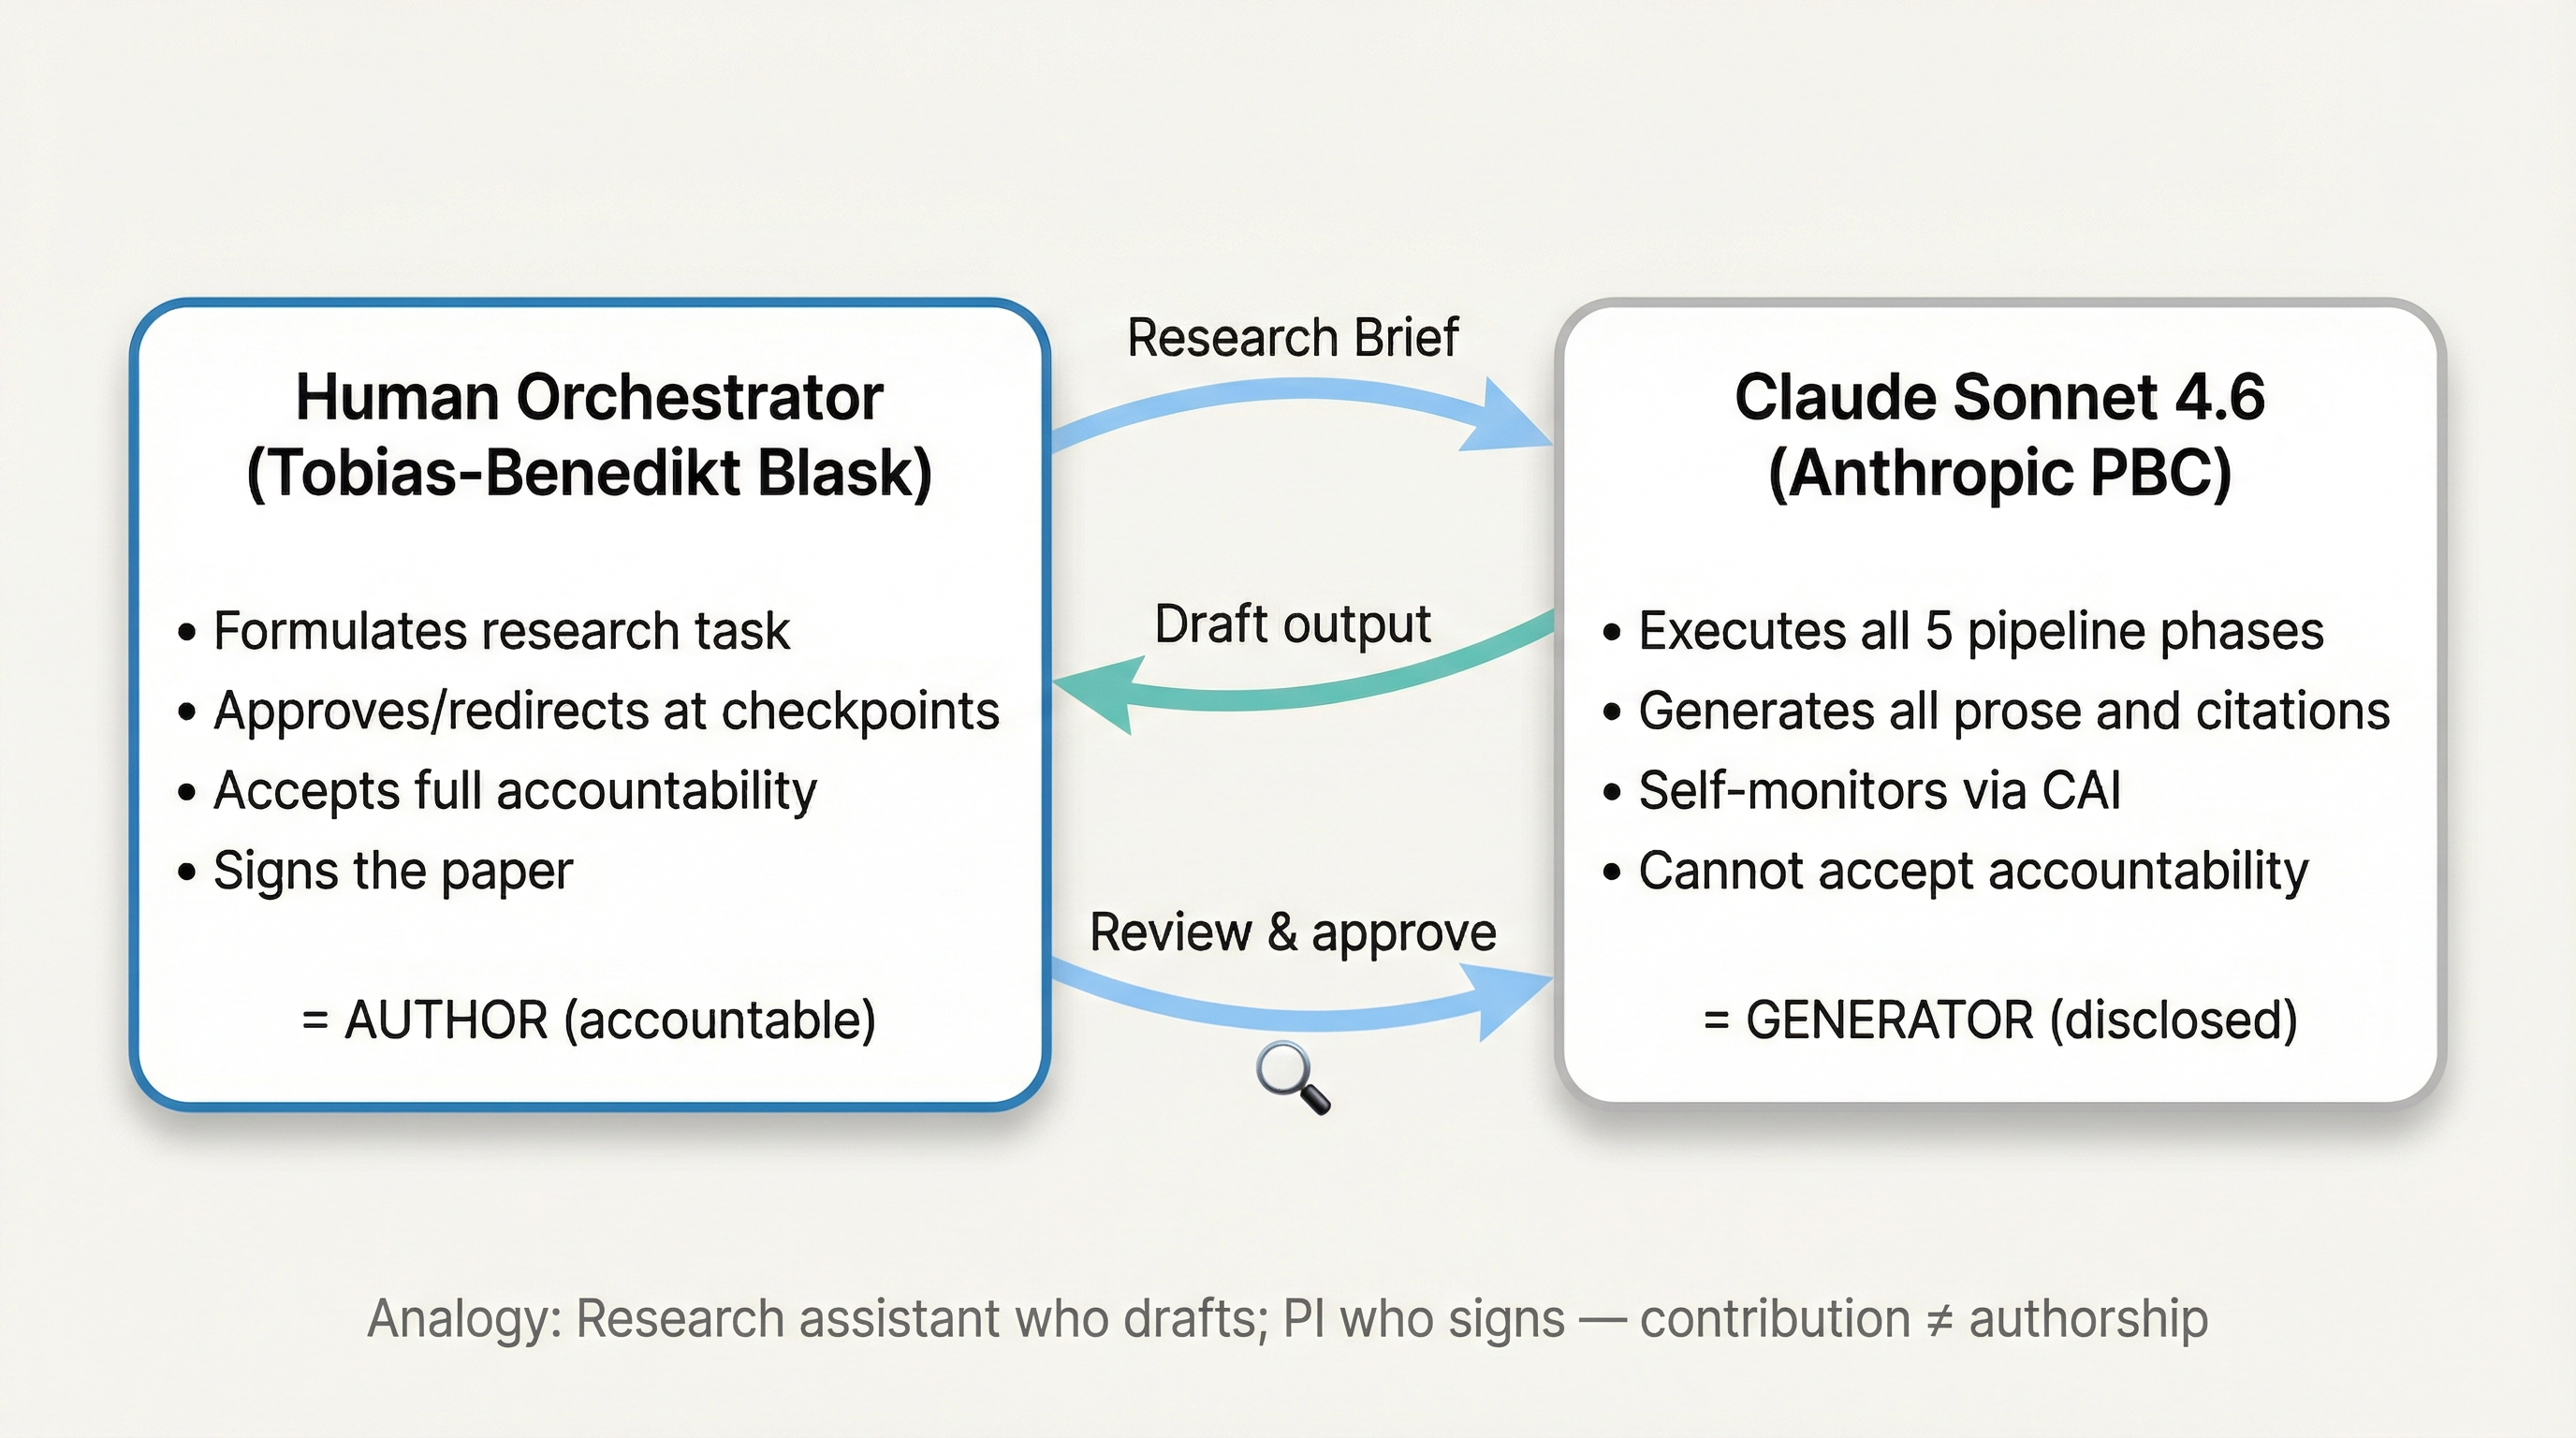
\includegraphics[width=0.9\textwidth]{figures/fig10_orchestrator_model.png}
    \caption{Accountability-based authorship under the orchestrator model. The human author provides direction to the AI system, evaluates its outputs, and accepts full responsibility for the published content. The AI system is disclosed as generator with all production artifacts archived for audit. Contribution disclosure replaces binary authorship attribution (cf.\ Section~6.3). Based on \citeauthor{asatiani2021envelopment}'s~(\citeyear{asatiani2021envelopment}) sociotechnical envelopment framework.}
    \label{fig:authorship_framework}
\end{figure}

\subsection{Peer Review in the Orchestrator Age}

If AI can produce papers that cite real literature, follow conventions, and advance plausible arguments, surface-level peer review becomes insufficient. \citet{mokander2023auditing} articulate the broader auditing challenge for LLMs.

The transition enables a complementary response: AI-augmented peer review.

\begin{itemize}
  \item \textbf{Citation verification:} Checking every cited paper against live databases, confirming existence and claimed content.
  \item \textbf{Hallucination detection:} Cross-referencing claims against retrieved source material.
  \item \textbf{Pipeline auditing:} Reviewing production artifacts for transparency and reproducibility.
  \item \textbf{Novelty assessment:} Comparing generated arguments against the existing literature to assess genuine contribution versus fluent recombination.
\end{itemize}

\citet{weng2024cycleresearcher} demonstrate automated research-review feedback loops. The Open Paper Machine incorporates a version of this principle: Phase~6 (Self-Review) generates a simulated peer review that the orchestrator uses to identify revision targets before submission. This is not automated quality assurance---the orchestrator must evaluate which critiques are valid---but it closes the feedback loop within the production pipeline. The archived artifacts---literature base, BibTeX, concept matrix, draft history, and self-review---model how AI-generated research might be made auditable. Transparency about the production process should be required for AI-assisted submissions, analogous to data availability requirements.

\subsection{The Research Scientist's Evolving Role}

The creator-to-orchestrator transition does not eliminate the research scientist. It restructures the role. Three dimensions of restructuring deserve attention.

\textbf{Epistemic judgment becomes more important, not less.} When AI generates fluent, convention-following prose, the scarce resource is no longer the ability to write---it is the ability to evaluate what is written. Distinguishing genuinely insightful synthesis from fluent recombination requires deep domain knowledge, theoretical sophistication, and what we might call \textit{epistemic taste}---an aesthetic sense for which arguments are productive and which are merely competent. This capacity develops through years of scholarly immersion, not through tool operation.

\textbf{Domain expertise intensifies.} The orchestrator cannot evaluate what they do not understand. Delegating literature search to an AI requires knowing the field well enough to recognize when the search has missed a critical strand. Delegating theoretical framing requires understanding the landscape of available theories well enough to judge whether the AI's selection is appropriate. The paradox: effective orchestration requires more domain expertise than manual execution, because the human must operate at a meta-level---evaluating process and output simultaneously.

\textbf{Institutional knowledge becomes essential.} Research is not merely cognitive work. It is institutionally embedded: conferences have norms, journals have preferences, reviewers have expectations, funding bodies have priorities. This institutional knowledge---knowing which arguments will land at ICIS versus MISQ, how to frame a contribution for a European versus American audience, when to be provocative and when to be conservative---is not learnable from training data. It requires the kind of socialization that doctoral programs, research groups, and conference communities provide.

\citet{scarbrough2024epistemic} show empirically that professionals make sense of AI differently based on their role identities. Applied to academia: a methods specialist may view the Open Paper Machine as a tool that amplifies their analytical reach; a theorist may view it as a threat to the craft of argumentation; a department chair may view it as a productivity enhancement or a quality risk. The orchestrator transition will be experienced differently across these professional identities.

\citet{degallier2022augmentation} argue for ``augmentation, not replacement'' as a design principle for AI in industry. We extend this to research: the Open Paper Machine augments the researcher's capacity to survey literature, generate drafts, and produce figures. It does not replace the researcher's capacity to formulate questions, evaluate arguments, design studies, or take accountability for claims.

% [R2-54: §6.6 Broader Transition deleted per Burkhardt R2 — "sehr breit am Ende"]
% Note: Fig 6 (capability matrix) moved to Section 5 where it fits better.

% [R2-55: §6.7 Research Agenda deleted per Burkhardt R2 — "würde die erstmal fallen lassen"]

% ============================================================
% [R2-48: Ethical Considerations relocated here from §3.4]
\section{Ethical Considerations}
\label{sec:ethics}

The reflexive design---an AI system analyzing its own production---raises distinctive ethical questions.

\textbf{Authorship.} The authors (Blask and Funk) take full responsibility for the published content. Claude Opus 4.6 is disclosed as the text generator. The system cannot accept moral or legal accountability, and current norms \citep{flanagin2023nonhuman} preclude AI authorship. This is not merely a pragmatic accommodation---it instantiates the orchestrator model: the human retains accountability precisely because the human retains evaluative authority.

\textbf{Integrity.} AI-generated papers raise questions about fabrication, hallucinated citations, and contribution to the scholarly record \citep{cotton2023cheating,kendall2024risks}. We address these through full disclosure, citation verification, and artifact archiving.

\textbf{Bias.} The system inherits biases from training data and RLHF evaluators. Literature selection over-represents English-language, Western, computationally-oriented sources. This is a structural limitation, not a correctable error.

% ============================================================
\section{Conclusion}
\label{sec:conclusion}

\subsection{Summary}

Two questions, two contributions. RQ1: the Open Paper Machine provides an architectural blueprint for LLM-based research pipelines, demonstrating full-pipeline execution---from literature search through \LaTeX{} compilation---while exhibiting fundamental limitations: hallucination risk, training cutoff, overconfident synthesis, no primary data generation, and evaluation bias. The reflexive analysis of this paper's own production documents both the capabilities and the failure modes. RQ2: the creator-to-orchestrator transition restructures the research scientist's role from text producer to process director, output evaluator, and accountability holder. This transition follows the task-based logic identified by \citet{autor2015why} and \citet{acemoglu2018automation}: execution tasks are delegated, judgment tasks intensify, and new orchestration tasks emerge. The transition is partial, not total---human ideas, epistemic judgment, and institutional knowledge remain irreplaceable.

% [R2-58: CRediT-based guidelines and Orchestration Trace added]
\subsection{Toward Practical Guidelines: CRediT and the Orchestration Trace}

The creator-to-orchestrator transition demands practical tools, not only theoretical frameworks. We propose two complementary instruments.

\textbf{CRediT-based AI contribution disclosure.} The Contributor Roles Taxonomy \citep{brand2015credit} defines 14 research contribution roles (Conceptualization, Methodology, Writing -- Original Draft, etc.). We propose extending CRediT to accommodate AI generators: for each role, authors would disclose whether the contribution was \textit{human-led}, \textit{AI-generated with human review}, or \textit{AI-generated with human revision}. For this paper, a CRediT-style disclosure would read: Conceptualization (human-led), Methodology (human-led), Software (AI-generated with human review), Formal Analysis (AI-generated with human revision), Writing -- Original Draft (AI-generated with human revision), Writing -- Review \& Editing (human-led), Visualization (AI-generated with human review), Supervision (human-led). This granularity replaces the binary ``AI-assisted yes/no'' with a structured account of the human--AI division of labor.

\textbf{The Orchestration Trace.} Beyond CRediT disclosure, we propose that AI-assisted papers archive an \textit{orchestration trace}: a structured record of (a)~the prompts and directives the human orchestrator provided, (b)~the points where human judgment overrode AI output, (c)~the verification steps applied to AI-generated content, and (d)~the final accountability assignment for each section. The Open Paper Machine implements a first version of the orchestration trace as a persistent log file (\texttt{orchestration\_log.md}) written throughout the production process. Each entry records a timestamp, the pipeline phase, the actor (human orchestrator or AI agent), the action type (generation, quality gate, redirect, verification), and the orchestrator's feedback. The log is designed for publication alongside the manuscript---for example, in a GitHub repository---making the human--AI division of labor auditable and comparable across papers. We recognize that a fully formalized orchestration trace standard would require community-level consensus---this paper offers the concept and a working implementation, not a finished specification.

Together, CRediT disclosure and the orchestration trace operationalize the accountability-based authorship model proposed in Section~\ref{sec:orchestrator}: they make the human--AI division of labor transparent, auditable, and comparable across papers.

\subsection{The Hard Problem}

The technology is ready. The institutions are not. The hard problem is not whether AI can produce research-quality manuscripts---this paper demonstrates that it can, within documented constraints. The hard problem is redesigning the institutional infrastructure: authorship norms, peer review processes, doctoral training programs, funding criteria, and promotion standards.

\citet{trist1951social} showed seventy-five years ago that mechanization without organizational redesign produces dysfunction. \citet{asatiani2021envelopment} translate this for AI: inscrutable systems require sociotechnical envelopment. The research community has a window---narrow, closing---to design the enveloping structures proactively rather than retrofitting them after dysfunction has already propagated.

\subsection{On Writing About Oneself}

This conclusion was generated by the system it describes. The irony is intended and inescapable. The system cannot evaluate its own output with detachment. Its self-assessment is shaped by the same training that produced the capabilities assessed. Its limitation acknowledgments are products of Constitutional AI---and may be systematically incomplete in ways the system cannot detect.

But the orchestrator is present. The human author evaluated this conclusion, compared it against the argument's trajectory, verified its citations, and approved its publication. The system generated the text; the human takes responsibility for the claims. This division---generation versus accountability---is the creator-to-orchestrator transition made concrete.

What this paper demonstrates is not that AI has achieved scientific understanding. It has not. What it demonstrates is that the mechanical phases of scientific production---the literature searches, the first drafts, the structured arguments---are becoming delegable. The irreducibly human contribution is not the production of text. It is the judgment that directs, evaluates, and takes responsibility for that text. The transition from creator to orchestrator does not diminish the researcher. It clarifies what the researcher has always been: not a text-production machine, but a judgment-bearing agent embedded in an epistemic community.

\vspace{1.5em}
\noindent\rule{\textwidth}{0.4pt}
\vspace{0.5em}
\noindent\textit{This paper was generated by Claude Opus 4.6 (Anthropic PBC) under orchestration by Tobias-Benedikt Blask (Harz University of Applied Sciences) and Burkhardt Funk (Leuphana University). The authors designed the research, evaluated all outputs, verified citations, and accept full responsibility for the published content. All pipeline artifacts are archived at \url{https://github.com/ProfDrT/From_Creator_to_Orchestrator}. The Open Paper Machine plugin is available at \url{https://github.com/ProfDrT/open-paper-machine}.}

% ============================================================
% APPENDIX
% ============================================================
% ============================================================
% APPENDIX — Production Artifacts and Workflow Documentation
% ============================================================

\appendix

% [R2-56: Appendix scope narrowed to OPM-specific content only]
\section{Plugin Architecture: The Open Paper Machine}
\label{app:plugin}

This appendix documents the \textit{Open Paper Machine specifically}---its plugin structure and orchestration dialogue. For general background on transformer architecture, RLHF, and Constitutional AI, see Section~\ref{sec:tech}.

The Open Paper Machine is a Claude Code plugin comprising 3{,}938 lines of prompt engineering, orchestration logic, and conversion utilities distributed across 18 files. The complete source is archived at \url{https://github.com/TobiasBlask/open-paper-machine}.

\subsection{System Overview}

The plugin consists of four architectural layers:

\begin{enumerate}
  \item \textbf{Plugin manifest} (\texttt{plugin.json}, 18 lines). Declares two MCP server dependencies: \texttt{academic-search} (Semantic Scholar, OpenAlex, CrossRef, arXiv APIs) and \texttt{paperbanana} (AI figure generation via Google Gemini). Both servers start automatically when Claude Code loads the plugin.

  \item \textbf{Autonomous agent} (\texttt{agents/paper-machine.md}, 570 lines). The core orchestration prompt that drives the six-phase pipeline. Operates on five principles: (1)~\textit{Do, don't ask}---make decisions and present results; (2)~\textit{Produce text, not plans}---every phase yields deliverable output; (3)~\textit{Checkpoint, don't block}---present work, then continue; (4)~\textit{Be explicit about decisions}---state what was chosen and why; (5)~\textit{Save everything to files}---every phase produces artifacts.

  \item \textbf{Skill engines} (7 modules, 1{,}933 lines total). Specialized execution modules activated on demand by the agent or user commands. Each encapsulates domain knowledge via fill-in-the-blank templates rather than abstract advice. Table~\ref{tab:skills} summarizes all engines.

  \item \textbf{Command interfaces} (8 commands, 685 lines total). User-facing entry points (\texttt{/write-paper}, \texttt{/search-papers}, \texttt{/export-latex}, \texttt{/verify-citations}, \texttt{/draft-section}, \texttt{/generate-figure}, \texttt{/generate-plot}, \texttt{/respond-reviewers}) that activate specific skill engines or the full pipeline.
\end{enumerate}

\begin{table}[H]
\centering
\small
\caption{Skill engines of the Open Paper Machine plugin.}
\label{tab:skills}
\begin{tabular}{@{}llp{7.5cm}@{}}
\toprule
\textbf{Engine} & \textbf{Lines} & \textbf{Capability} \\
\midrule
writing-engine & 339 & Sentence, paragraph, and section templates for IS/WI/BWL research. Provides concrete fill-in-the-blank formulas (e.g., 6-paragraph introduction blueprint, IMRAD section patterns). \\
literature-engine & 213 & API-first literature discovery across four academic databases. Search strategy generation, concept matrix construction, citation snowballing, narrative synthesis. \\
theory-engine & 169 & Theory selection (TOE, UTAUT, Dynamic Capabilities, etc.), research gap formulation, hypothesis derivation, contribution statement templates. \\
method-engine & 353 & Methodology decision trees for SLR, case study, Gioia, Mayring, grounded theory, PLS-SEM, DSR, and mixed methods. Complete method section templates. \\
figure-engine & 202 & AI figure generation via PaperBanana MCP (Gemini backend) with matplotlib/seaborn fallback. Transforms text descriptions into publication-quality diagrams. \\
latex-engine & 281 & Markdown-to-LaTeX conversion, \texttt{\textbackslash citep}/\texttt{\textbackslash citet} resolution, booktabs tables, arxiv-style compilation. Uses \texttt{md\_to\_latex.py} (732 lines). \\
verification-engine & 376 & Citation verification against source abstracts and full-text. Classifies each citation as VERIFIED, PLAUSIBLE, MISMATCH, UNVERIFIABLE, or NOT FOUND. \\
\bottomrule
\end{tabular}
\end{table}

\subsection{Artifact Inventory}

The pipeline produces the following intermediate artifacts, all version-controlled in the repository:

\begin{itemize}
  \item \texttt{literature\_base.csv} --- Retrieved literature database (Phase 1)
  \item \texttt{references.bib} --- BibTeX entries for all cited papers (Phase 1)
  \item \texttt{framing.md} --- Theory selection, gap formulation, research questions (Phase 2)
  \item \texttt{concept\_matrix.md} --- Webster \& Watson concept matrix (Phase 3)
  \item \texttt{paper\_structure.md} --- Section structure with word budget (Phase 3)
  \item \texttt{draft.md} --- Complete paper draft as Markdown (Phase 4)
  \item \texttt{figures/} --- PaperBanana-generated diagrams, 300 DPI PNG (Phase 5)
  \item \texttt{latex/paper.tex} --- arxiv-style LaTeX source (Phase 5)
  \item \texttt{latex/paper.pdf} --- Compiled PDF manuscript (Phase 5)
  \item \texttt{status\_report.md} --- Self-assessed completion status (Phase 6)
  \item \texttt{verification\_report.md} --- Citation verification results (optional Phase 7)
\end{itemize}

% [R3: Appendix B (Prototypical Dialogue) deleted per Burkhardt — orchestrator role appeared too passive in the example]

% ============================================================
\section{Orchestrator--Agent Interaction Timeline}
\label{app:timeline}

This appendix documents the complete sequence of substantive orchestrator--agent interactions during the production of this paper. Each entry records the pipeline phase, the \textit{character} of the interaction (approval, redirect, expansion, correction, or evaluation), and what it reveals about the orchestrator role. Routine interactions (``proceed,'' ``looks good'') are omitted; only interactions that shaped the paper's content or direction are included.

\vspace{0.5em}

\begin{table}[H]
\centering
\small
\caption{Orchestrator--agent interaction timeline. Character types: \textbf{D}~= Direction (new task or redirect), \textbf{E}~= Expansion (add scope), \textbf{C}~= Correction (fix error), \textbf{V}~= Evaluation (quality judgment), \textbf{A}~= Approval (gate passed).}
\label{tab:timeline}
\begin{tabularx}{\textwidth}{@{} c l c X @{}}
\toprule
\textbf{\#} & \textbf{Phase} & \textbf{Char.} & \textbf{Interaction} \\
\midrule
1 & Phase 1 & D & \textit{Orchestrator} initiates pipeline with title and research topic. Agent autonomously executes 6 search queries across 4 databases, returns 171 candidates. \\[0.3em]
2 & Phase 1 & E & \textit{Orchestrator} judges sociotechnical theory coverage as thin. Commissions 3 additional targeted searches (``sociotechnical envelopment AI,'' ``task-based automation framework,'' ``distributed cognition AI systems''), adding 14 papers. \\[0.3em]
3 & Phase 1 & A & Corpus approved: 62 papers retained for concept matrix. \\[0.3em]
4 & Phase 2 & D & \textbf{Key redirect.} Agent frames paper as pure systems description. \textit{Orchestrator rejects} and redirects toward creator-to-orchestrator thesis---the substantive intellectual decision that shaped the entire argument. \\[0.3em]
5 & Phase 2 & V & \textit{Orchestrator} evaluates theory selection (distributed cognition, sociotechnical systems, Autor). Approves combination; adds Scarbrough (2024) as missing empirical complement. \\[0.3em]
6 & Phase 3 & V & \textit{Orchestrator} reviews section structure. Rebalances word budget: reduces technology description (\S4), expands discussion (\S6). \\[0.3em]
7 & Phase 3 & A & Structure approved: 8 sections, $\sim$10{,}000 words. \\[0.3em]
8 & Phase 4 & C & \textit{Orchestrator} spot-checks citations against retrieved abstracts. Identifies 4 hallucinated claims (correct paper, incorrect attributed finding). Agent corrects. \\[0.3em]
9 & Phase 4 & V & \textit{Orchestrator} evaluates prose quality. Flags ``intellectual risk'' deficit: too hedged, too balanced. Instructs agent to sharpen provocative arguments (esp.\ \S6.2 desk research). \\[0.3em]
10 & Phase 5 & C & \textbf{Figure correction.} Co-author identifies conceptual error: ``accountability'' arrow from AI System to Published Output contradicts core argument. Agent confirms error, regenerates figure. \\[0.3em]
11 & Phase 5 & A & \LaTeX{} compilation approved. All figures, tables, references resolve. \\[0.3em]
12 & Phase 6 & V & Agent generates self-review (simulated peer review). \textit{Orchestrator} evaluates 12 critique points: accepts 8, rejects 4 as unfounded. Accepted critiques drive final revision pass. \\[0.3em]
13 & Co-author & D & Co-author review introduces new requirements: position paper framing, shorter \S4, ``desk research $\rightarrow$ desk reject'' argument. Agent implements; orchestrator verifies. \\[0.3em]
14 & R2 Revision & E & 59 review comments processed. Agent drafts responses and edits; orchestrator evaluates each for argumentative coherence and reviewer intent. \\
\bottomrule
\end{tabularx}
\end{table}

\subsection{Patterns in the Interaction}

Three patterns emerge from the timeline:

\begin{enumerate}
    \item \textbf{The orchestrator's most consequential interventions are redirections, not corrections.} Interaction \#4 (rejecting the systems framing in favor of the creator-to-orchestrator thesis) shaped the entire paper more than any error correction. This is the ``step up'' strategy \citep{davenport2016just}: the orchestrator operates at the level of research direction, not prose production.

    \item \textbf{Corrections cluster at the semantic level, not the syntactic level.} The agent produces grammatically correct, convention-following prose. Errors occur at the level of \textit{meaning}: hallucinated claims (\#8), conceptual contradictions in figures (\#10), insufficient intellectual risk (\#9). These are precisely the errors that require domain expertise to detect.

    \item \textbf{The interaction character shifts across phases.} Early phases are dominated by \textit{direction} and \textit{expansion} (what to research, how to frame it). Middle phases shift to \textit{correction} and \textit{evaluation} (are the claims right? is the prose sharp enough?). Late phases return to \textit{direction} as co-author feedback introduces new requirements. This pattern---\textit{direct} $\rightarrow$ \textit{evaluate} $\rightarrow$ \textit{redirect}---mirrors the orchestrator cycle depicted in Figure~\ref{fig:creator_to_orchestrator}.
\end{enumerate}

\subsection{What the Timeline Reveals}

The timeline operationalizes the ``orchestration is substantive intellectual work'' claim from Section~3.2. Across 14 substantive interactions, the orchestrator:
\begin{itemize}[nosep]
    \item Made 3 directional decisions that shaped the paper's argument (\#1, \#4, \#13)
    \item Expanded scope based on domain knowledge 2 times (\#2, \#14)
    \item Corrected semantic errors the agent could not self-detect 2 times (\#8, \#10)
    \item Exercised evaluative judgment on quality, balance, and sharpness 4 times (\#5, \#6, \#9, \#12)
\end{itemize}

\noindent None of these interactions involved text production. All involved judgment. This is the creator-to-orchestrator transition made observable.

% End of appendix content


% ============================================================
% [R2-59: Switched to APA-like bibliography style]
\bibliographystyle{apalike}
\bibliography{references}

\end{document}
